\section{DODATEK B: Dokumentacja techniczna}
\label{sub:dodatekB}

Projekt został napisany w programie \textit{MATLAB 2017b}. Korzystano z gotowego GUI programu \textit{MATLAB - Neural Network Toolbox} oraz innych funkcji z tego \textit{toolbox}. Baza danych potrzebna do realizacji postawionego zadania została pobrana z źródła \cite{baza_down}.

\subsection{Dokumentacja oprogramowania}
\label{sub:dokumentacja}

Wszystkie funkcje użyte na potrzeby zaimplementowania algorytmu zostały zaczerpnięte z gotowych rozwiązań. Opis i dokumentacja techniczna GUI \textit{Neural Network Toolbox} znajduje się w źródle \cite{gui}, zaś do funkcji użytych w procesie tworzenia głębokich sieci neuronowych w źródle \cite{funkcje}.

\noindent Kolejność użytych funkcji przedstawiono na schemacie \ref{fig:flow}. Dokładne omówienie kodu znajduje się poniżej.

\vspace{0.6cm}

\begin{figure}[H]
	\centering
	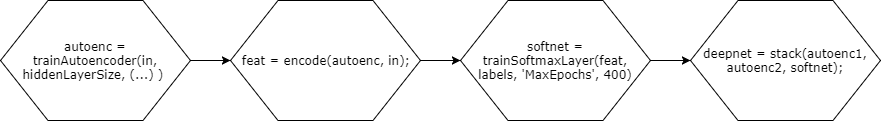
\includegraphics[scale=0.45]{obrazki/flow}
	\caption{\label{fig:subcaption_example}Schemat blokowy użytych funkcji do głębokiego uczenia sieci neuronowej.}{\label{fig:flow}}
\end{figure}

\noindent Funkcja \textit{trainAutoencoder} tworzy ukryte warstwy o zadanej liczbie neuronów. Jako parametry przyjmuje dane wejściowe, ilość ukrytych neuronów oraz parametry określające dynamikę i właściwości wag. Dodatkowo można tu zdecydować, czy obliczenia mają być wykonywane również na procesorze GPU. Funkcja \textit{encode} służy do ekstrakcji cech z~ukrytych warstw, a jako parametry przyjmuje dane wejściowe oraz wynik działania auto-enkodera. Funkcja \textit{trainSoftmaxLayer} tworzy funkcję aktywacji typu softmax, bazując na cechach zwróconych po wywołaniu funkcji \textit{encode} oraz etykietach danych wejściowych. Określa się tutaj także maksymalną liczbę epok. Ostatnia funkcja \textit{stack} układa wszystkie warstwy, łącząc stworzone auto-enkodery oraz warstwę wyjściową. Funkcja ta tworzy głęboką sieć neuronową, która może być już użyta do testowania.


\noindent Dokumentacja techniczna do każdej użytej funkcji znajduje się poniżej.

\vspace{1cm}
\hrule
\vspace{1cm}

\noindent data = dat2mat(['path' '.aedat']);
\vspace{1cm}

\noindent \textit{@file} Skrypt programu \textit{MATLAB} napisany przez twórców\cite{MNIST_DVS} bazy \textit{MNIST-DVS} do zamiany formatu danych .aedat na format .mat akceptowany i widziany przez \textit{MATLAB}.
\\ \textit{@param} ['path' '.aedat'] Ścieżka do danych w formacie .aedat.
\\ \textit{@return} data Wynik działania skryptu. Przedstawienie danych podanych jako parametr w formacie .mat.

\vspace{1cm}
\hrule
\vspace{1cm}

\noindent [trainInd,valInd,testInd] = dividerand(length(images), trainRatio, valRatio, testRatio);
\vspace{1cm}

\noindent \textit{@fn} dividerand Funkcja dzieli określony ciąg liczb na trzy grupy używając losowych indeksów. W przypadku rozważanego algorytmu funkcja umożliwiła losowy podział zbioru wejściowego na zbiór: uczący, walidacyjny i testowy.
\\ \textit{@param} length(images) Liczba określająca wielkość zbioru, który ulega podziałowi. Tu: wielkość bazy danych wejściowych.
\\ \textit{@param} trainRatio Stosunek procentowy udziału danych w zbiorze treningowym. Default = 0.7.
\\ \textit{@param} valRatio Stosunek procentowy udziału danych w zbiorze walidacyjnym. Default = 0.15.
\\ \textit{@param} testRatio Stosunek procentowy udziału danych w zbiorze testowym. Default = 0.15.
\\ \textit{@return} trainInd Wektor indeksów danych treningowych.
\\ \textit{@return} valInd Wektor indeksów danych walidacyjnych.
\\ \textit{@return} testInd Wektor indeksów danych testowych.

\vspace{1cm}
\hrule
\vspace{1cm}

\noindent autoenc1 = trainAutoencoder(images$\_$train,hiddenSize1, ...
\\ \indent   'MaxEpochs',400, ...
\\ \indent   'L2WeightRegularization',0.004, ...
\\ \indent   'SparsityRegularization',4, ...
\\ \indent   'SparsityProportion',0.15, ...
\\ \indent   'ScaleData', false, ...
\\ \indent   'useGPU',true);
\vspace{1cm}

\noindent \textit{@fn} trainAutoencoder Funkcja trenuje auto-enkoder o zadanej liczbie neuronów ukrytych i kluczowych parametrach z punktu widzenia budowy sieci i użycia zasobów sprzętowych.
\\ \textit{@param} images$\_$train Zbiór danych uczących w przypadku pierwszej warstwy ukrytej. W przypadku tworzenia kolejnych warstw (w rozważanym zadaniu użyto dwóch auto-enkoderów) jest to zbiór wyjściowy danych z poprzedniej warstwy ukrytej. Dane powinny być wyrażone w postaci macierzy lub tablicy celek. W każdym z przypadków dane powinny znajdować się w kolumnach bądź poszczególnych celkach o takim samym rozmiarze.
\\ \textit{@param} hiddenSize1 Liczba neuronów w warstwie ukrytej, jest to dodatnia wartość typu integer. Default = 10.
\\ \textit{@param} 'MaxEpochs' Maksymalna liczba epok treningowych, jest to dodatnia wartość typu integer. Default = 1000.
\\ \textit{@param} 'L2WeightRegularization' Współczynnik dla regulacji wag. Regulacja ta pozwala na uniknięcie zbytniego wzrostu wartości wag na rzecz wyjścia. Powoduje wyskalowanie tego parametru w funkcji kosztu. Jest to dodatnia wartość skalarna. Default = 0.001.
\\ \textit{@param} 'SparsityRegularization' Współczynnik kontrolujący wpływ parametru odpowiedzialnego za regulację wartości aktywacji neuronów w funkcji kosztu. Jest to dodatnia wartość skalarna. Default = 1.
\\ \textit{@param} 'SparsityProportion' Wskaźnik określający na ile przykładów danych treningowych ma reagować neuron. Im ta wartość jest mniejsza, tym neuron na mniej danych wejściowych będzie reagował wysokim wyjściem. Jest to dodatnia wartość skalarna z~zakresu 0 - 1. Default = 0.05.
\\ \textit{@param} 'ScaleData' Parametr odpowiedzialny za skalowanie rozmiarem danych w auto-enkoderze automatycznie, co powoduje, że wejścia są replikowane na wyjścia. Przyjmuje wartość true lub false. Default = true.
\\ \textit{@param} 'useGPU' Parametr określający użycie GPU podczas trenowania. Przyjmuje wartość true lub false. Default = false.
\\ \textit{@return} autoenc1 Auto-enkoder stworzony z zadanymi parametrami, wytrenowany za pomocą danych wejściowych images$\_$train.

\vspace{1cm}
\hrule
\vspace{1cm}

\noindent plotWeights(autoenc1);
\vspace{1cm}

\noindent \textit{@fn} plotWeights Funkcja wyświetlająca wagi dla neuronów ukrytych. Funkcja nie zwraca żadnych wartości, ale w wyniku jej działania na ekranie pojawia się wykres.
\\ \textit{@param} autoenc1 Auto-enkoder stworzony i wytrenowany za pomocą funkcji \textit{trainAutoencoder}.

\vspace{1cm}
\hrule
\vspace{1cm}

\noindent feat1 = encode(autoenc1, images$\_$train);
\vspace{1cm}

\noindent \textit{@fn} encode Funkcja tworzy i zwraca zakodowane dane, podane jako parametr, używając wytrenowanego wcześniej auto-enkodera. Dane te mogą być później wykorzystane jako wejście do kolejnych warstw ukrytych lub warstwy wyjściowej.
\\ \textit{@param} autoenc1 Auto-enkoder stworzony i wytrenowany za pomocą funkcji \textit{trainAutoencoder}.
\\ \textit{@param} images$\_$train Zbiór danych uczących w przypadku pierwszej warstwy ukrytej. W przypadku tworzenia kolejnych warstw (w rozważanym zadaniu użyto dwóch auto-enkoderów) jest to zbiór wyjściowy danych z poprzedniej warstwy ukrytej. Dane powinny być wyrażone w postaci macierzy lub tablicy celek. W każdym z przypadków dane powinny znajdować się w kolumnach bądź poszczególnych celkach o takim samym rozmiarze. Format tych danych zależy od tego, na jakim formacie danych trenowany był auto-enkoder.
\\ \textit{@return} feat1 Dane zakodowane za pomocą auto-enkodera i wyrażone w postaci macierzy. To cechy wygenerowane z danych wejściowych. Każda dana reprezentuje osobną kolumnę, ilość wierszy wskazuje na ilość neuronów ukrytych w auto-enkoderze.

\vspace{1cm}
\hrule
\vspace{1cm}

\noindent labels$\_$train$\_$temp{i} = reshape(labels$\_$train{i}, [size$\_$x,size$\_$y]);
\vspace{1cm}

\noindent \textit{@fn} reshape Funkcja powoduje utworzenie nowej tablicy poprzez zmianę wymiarów tablicy już istniejącej.
\\ \textit{@param} labels$\_$train{i} Tablica wzorcowa, która zostaje poddana zmianie rozmiaru.
\\ \textit{@param} [size$\_$x,size$\_$y] Nowy rozmiar tablicy.
\\ \textit{@return} labels$\_$train$\_$temp{i} Miejsce, w którym zostanie zapisana nowa tablica.

\vspace{1cm}
\hrule
\vspace{1cm}

\noindent labels$\_$train3 = cell2mat(labels$\_$train$\_$temp);
\vspace{1cm}

\noindent \textit{@fn} cell2mat Funkcja konwertująca tablicę celek na standardową tablicę podstawowych typów.
\\ \textit{@param} labels$\_$train$\_$temp Tablica celek.
\\ \textit{@return} labels$\_$train3 Tablica standardowa, utworzona z elementów znajdujących się poprzednio w celkach.

\vspace{1cm}
\hrule
\vspace{1cm}

\noindent softnet = trainSoftmaxLayer(feat2, labels$\_$train3, 'MaxEpochs', 400);
\vspace{1cm}

\noindent \textit{@fn} trainSoftmaxLayer Funkcja stwarza warstwę wyjściową i klasyfikuje cechy z warstwy poprzedniej przy użyciu etykiet rzeczywistych.
\\ \textit{@param} feat2 Dane treningowe. Mogą to być zarówno dane wejściowe jak i cechy zwrócone przez poprzednią warstwę. W kolumnach znajdują się poszczególne próby, w~wierszach kolejne cechy.
\\ \textit{@param} labels$\_$train3 Rzeczywiste etykiety danych. Liczba wierszy specyfikuje liczbę klas, a więc wyjść z sieci, zaś każda kolumna specyfikuje kolejną daną. Trzeba zaznaczyć, że w danej kolumnie tylko jedna cyfra ma wartość 1, pozostałe mają wartość 0 i ta jedynka specyfikuje przynależność danej do tej konkretnej klasy. 
\\ \textit{@param} 'MaxEpochs' Maksymalna liczba epok treningowych, jest to dodatnia wartość typu integer. Default = 1000.
\\ \textit{@return} 

\vspace{1cm}
\hrule
\vspace{1cm}

\noindent deepnet = stack(autoenc1, autoenc2, softnet);
\vspace{1cm}

\noindent \textit{@fn} stack Funkcja układa w stos enkodery z kilku auto-enkoderów, tworząc pełną sieć neuronową.
\\ \textit{@param} autoenc1 Auto-enkoder pierwszy stworzony i wytrenowany za pomocą funkcji \textit{trainAutoencoder}.
\\ \textit{@param} autoenc2 Auto-enkoder drugi stworzony i wytrenowany za pomocą funkcji \textit{trainAutoencoder}.
\\ \textit{@param} softnet Warstwa wyjściowa stworzona za pomocą funkcji \textit{trainSoftmaxLayer}.
\\ \textit{@return} deepnet Obiekt sieci neuronowej składający się z enkoderów elementów określonych jako parametry funkcji.

\vspace{1cm}
\hrule
\vspace{1cm}

\noindent view(deepnet);
\vspace{1cm}

\noindent \textit{@fn} view Funkcja pokazująca strukturę sieci podanej jako parametr z określeniem ilości neuronów i warstw. Funkcja nie zwraca żadnych wartości, ale w wyniku jej działania na ekranie pojawia się diagram.
\\ \textit{@param} deepnet Obiekt sieci neuronowej stworzony na przykład za pomocą funkcji \textit{stack}.

\vspace{1cm}
\hrule
\vspace{1cm}

\noindent y = deepnet(xTest);
\vspace{1cm}

\noindent \textit{@fn} deepnet Wywołanie to pozwala na uzyskanie wyników działania sieci neuronowej na danych ze zbioru testowego. Używa tutaj stworzonego wcześniej obiektu sieci neuronowej deepnet.
\\ \textit{@param} xTest Zbiór danych wejściowych wyrażony jako tablica licz typu \textit{double}. Liczba wierszy stanowi o rozmiarze tych danych, liczba kolumn wskazuje na ich liczbę.
\\ \textit{@return} y Wynik działania sieci neuronowej. Jest to tablica, której liczba kolumn informuje o liczbie danych wejściowych, a liczba wierszy wskazuje na liczbę neuronów w~warstwie wyjściowej (i ich odpowiedzi dla danej o tym samym numerze kolumny).

\vspace{1cm}
\hrule
\vspace{1cm}

\noindent plotconfusion(labels$\_$test3, y);
\vspace{1cm}

\noindent \textit{@fn} plotconfusion Funkcja pozwala na odczytanie macierzy błędu, czyli zbadanie związku pomiędzy właściwą klasyfikacją danych wejściowych a tą, zwróconą przez sieć neuronową. Funkcja nie zwraca żadnej wartości, ale w wyniku jej działania na ekranie pojawia się macierz opisująca analizę ilościową i jakościową testów.
\\ \textit{@param} labels$\_$test3 Oryginalne etykiety danych poddanych testowaniu przez sieć.
\\ \textit{@param} y Etykiety wygenerowane przez sieć neuronową po przepuszczeniu przez nią danych testowych.

\vspace{1cm}
\hrule
\vspace{1cm}

\noindent deepnet = train(deepnet, xTrain, labels$\_$train3);
\vspace{1cm}

\noindent \textit{@fn} train Funkcja trenuje sieć neuronową zgodnie z zadanymi parametrami, wykorzystując metodę \textit{backpropagation}. Zwraca nową sieć, zmodyfikowaną sieć.
\\ \textit{@param} deepnet Obiekt sieci neuronowej stworzony na przykład za pomocą funkcji \textit{stack}
\\ \textit{@param} xTrain Dane treningowe. Dane znajdują się w macierzy liczb double o liczbie wierszy wskazującej na wielkość jednej danej, w kolejnych kolumnach znajdują się kolejne dane testowe.
\\ \textit{@param} labels$\_$train3 Oryginalne etykiety danych poddanych trenowaniu przez sieć. Etykiety znajdują się w poszczególnych wierszach, numer kolumny odpowiada danej, dla której została przyporządkowana etykieta.
\\ \textit{@return} deepnet Obiekt sieci neuronowej stworzony na przykład za pomocą funkcji \textit{train}, używający metody \textit{backpropagation} w procesie uczenia.

\vspace{1cm}
\hrule
\vspace{1cm}



\subsection{Procedura symulacji, testowania i weryfikacji}
\label{sub:procedura}

Do realizacji projektu nie używano żadnej zewnętrznej platformy sprzętowej. Aby uruchomić aplikację wystarczy komputer PC spełniający wymagania sprzętowo - programowe opisane w sekcji \ref{sub:przygotowanie} z zainstalowanym programem \textit{MATLAB 2017b}. Potrzebny jest także \textit{Neural Network Toolbox}, który będzie wbudowany w przypadku pełnej instalacji programu. W celu przygotowania danych do uczenia można pobrać bazę ze źródła \cite{baza} i uruchomić skrypt \textit{Data$\_$selection} znajdujący się na nośniku CD. Można również wczytać przygotowane już dane w formacie .mat: data$\_$matrix.mat oraz images$\_$double.mat znajdujące się również na nośniku CD. W celu weryfikacji algorytmu należy skorzystać z \textit{Neural Network Toolbox}, wybierając opcję \textit{Pattern recognition and classification}. Jako wejście należy wczytać macierze input$\_$matrix oraz output$\_$matrix. Druga opcja zakłada skorzystanie z głębokiego uczenia z użyciem większej liczby warstw ukrytych. W~tym celu trzeba uruchomić skrypt \textit{GPU$\_$Mnist} (płyta CD). Należy zaznaczyć, że proces trwa dosyć długo, a liczenie przebiega tu w sposób równoległy i z użyciem procesora graficznego GPU.

